%%%%%%%%%%%%%%%%%%%%%%%%%%%%%%%%%%%%%
%                                   %
% Compile with XeLaTeX and biber    %
%                                   %
% Questions or comments:            %
%                                   %
% joshua dot mcneill at uga dot edu %
%                                   %
%%%%%%%%%%%%%%%%%%%%%%%%%%%%%%%%%%%%%

\documentclass{beamer}
  % Read in standard preamble (cosmetic stuff)
  %%%%%%%%%%%%%%%%%%%%%%%%%%%%%%%%%%%%%%%%%%%%%%%%%%%%%%%%%%%%%%%%
% This is a standard preamble used in for all slide documents. %
% It basically contains cosmetic settings.                     %
%                                                              %
% Joshua McNeill                                               %
% joshua dot mcneill at uga dot edu                            %
%%%%%%%%%%%%%%%%%%%%%%%%%%%%%%%%%%%%%%%%%%%%%%%%%%%%%%%%%%%%%%%%

% Beamer settings
% \usetheme{Berkeley}
\usetheme{CambridgeUS}
% \usecolortheme{dove}
% \usecolortheme{rose}
\usecolortheme{seagull}
\usefonttheme{professionalfonts}
\usefonttheme{serif}
\setbeamertemplate{bibliography item}{}

% Packages and settings
\usepackage{fontspec}
  \setmainfont{Charis SIL}
\usepackage{hyperref}
  \hypersetup{colorlinks=true,
              allcolors=blue}
\usepackage{graphicx}
  \graphicspath{{../../figures/}}
\usepackage[normalem]{ulem}
\usepackage{enumerate}

% Document information
\author{M. McNeill}
\title[FREN2001]{Français 2001}
\institute{\url{joshua.mcneill@uga.edu}}
\date{}

%% Custom commands
% Lexical items
\newcommand{\lexi}[1]{\textit{#1}}
% Gloss
\newcommand{\gloss}[1]{`#1'}
\newcommand{\tinygloss}[1]{{\tiny`#1'}}
% Orthographic representations
\newcommand{\orth}[1]{$\langle$#1$\rangle$}
% Utterances (pragmatics)
\newcommand{\uttr}[1]{`#1'}
% Sentences (pragmatics)
\newcommand{\sent}[1]{\textit{#1}}
% Base dir for definitions
\newcommand{\defs}{../definitions}


  % Packages and settings

  % Document information
  \subtitle[Ma famille]{Voici ma famille}

\begin{document}
  % Read in the standard intro slides (title page and table of contents)
  \begin{frame}
    \titlepage
    \tiny{Office: % Basically a variable for office hours location
Gilbert 121\\
          Office hours: % Basically a variable for office hours
 lundi, mercredi, vendredi 10:10--11:10
}
  \end{frame}

  \begin{frame}{Annonces}
    \begin{enumerate}
      \item \gloss{MFL assignments must be completed by class time starting Monday.}
      \item \gloss{New assignment on eLC due September 12th (eLC > Tools > Assignments)}
      \item \gloss{Unauthorized Access paper signed and returned by Monday.}
    \end{enumerate}
  \end{frame}

  \begin{frame}{Arbre généalogique \gloss{Family tree}}
    \begin{columns}
      \column{0.5\textwidth}
        \uncover<2->{
          Les Simpson
        }
        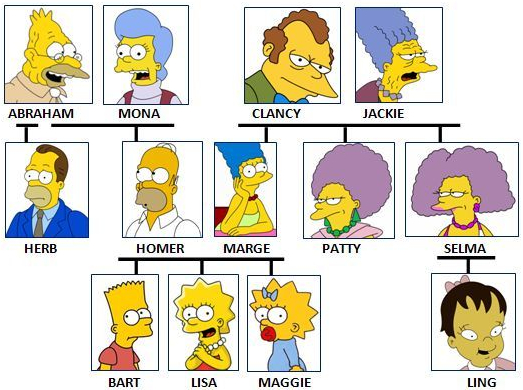
\includegraphics[scale=0.45]{simpsons.jpg}
      \column{0.5\textwidth}
      \begin{minipage}[t][0.6\textheight]{\linewidth}
        \vspace{14pt}
        \only<3-4>{
          Le père du père de Bart est \underline{\uncover<4->{son grand-père}}.
        }
        \only<5-6>{
          La fille de la mère de Marge est \underline{\uncover<6->{sa sœur}}.
        }
        \only<7-8>{
          Les filles du fils de Mona sont \underline{\uncover<8->{ses petites-filles}}.
        }
        \only<9-10>{
          La fille de la tante de Maggie est \underline{\uncover<10->{sa cousine}}.
        }
        \only<11-12>{
          Les parents de la mère de Lisa sont \underline{\uncover<12->{ses grands-parents}}.
        }
        \only<13-15>{
          Le fils de la mère du père de Bart est \underline{\uncover<14->{son oncle}}.
          \uncover<15->{
            \begin{center}
              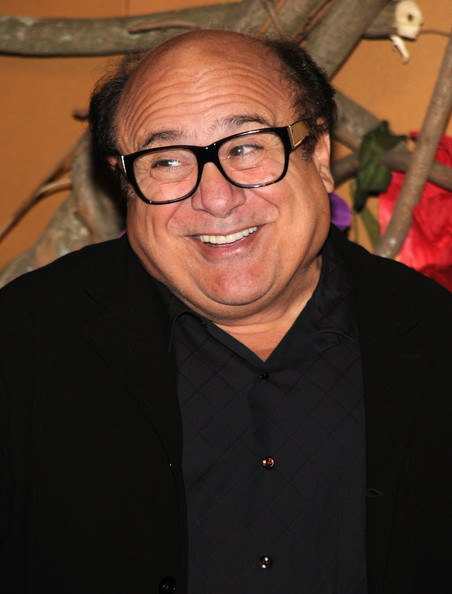
\includegraphics[scale=0.7]{devito.jpg}
            \end{center}
          }
        }
      \end{minipage}
    \end{columns}
  \end{frame}

  \begin{frame}{}
    \begin{center}
      \Large Quiz
    \end{center}
  \end{frame}

  % Preface this one by talking about your own extended family and spelling
  % the names.
  \begin{frame}{Comment ça s'écrit? \gloss{How is that spelled?}}
    \gloss{With a partner, share the last names that make up your extended family.
    For each last name, ask your partner how to spell the name and write it down.}
    \begin{itemize}
      \item[E1:] Dans ma famille, il y a des ..., des ... et des ...
      \item[E2:] Comment ... s'écrit?
      \item[E1:] Ça s'écrit ...
    \end{itemize}
  \end{frame}

  \begin{frame}{}
    \begin{center}
      \Large Questions?
    \end{center}
  \end{frame}
\end{document}
